\documentclass[10pt,ignorenonframetext,,aspectratio=149]{beamer}
\usefonttheme{serif} % use mainfont rather than sansfont for slide text
\setbeamertemplate{caption}[numbered]
\setbeamertemplate{caption label separator}{: }
\setbeamercolor{caption name}{fg=normal text.fg}
\usepackage{lmodern}
\usepackage{amssymb,amsmath}
\usepackage{ifxetex,ifluatex}
\usepackage{fixltx2e} % provides \textsubscript
\ifnum 0\ifxetex 1\fi\ifluatex 1\fi=0 % if pdftex
  \usepackage[T1]{fontenc}
  \usepackage[utf8]{inputenc}
\else % if luatex or xelatex
  \ifxetex
    \usepackage{mathspec}
  \else
    \usepackage{fontspec}
  \fi
  \defaultfontfeatures{Ligatures=TeX,Scale=MatchLowercase}
  \newcommand{\euro}{€}
    \setmainfont[]{Open Sans}
\fi
% use upquote if available, for straight quotes in verbatim environments
\IfFileExists{upquote.sty}{\usepackage{upquote}}{}
% use microtype if available
\IfFileExists{microtype.sty}{%
\usepackage{microtype}
\UseMicrotypeSet[protrusion]{basicmath} % disable protrusion for tt fonts
}{}
\usepackage{color}
\usepackage{fancyvrb}
\newcommand{\VerbBar}{|}
\newcommand{\VERB}{\Verb[commandchars=\\\{\}]}
\DefineVerbatimEnvironment{Highlighting}{Verbatim}{commandchars=\\\{\}}
% Add ',fontsize=\small' for more characters per line
\usepackage{framed}
\definecolor{shadecolor}{RGB}{248,248,248}
\newenvironment{Shaded}{\begin{snugshade}}{\end{snugshade}}
\newcommand{\AlertTok}[1]{\textcolor[rgb]{0.94,0.16,0.16}{#1}}
\newcommand{\AnnotationTok}[1]{\textcolor[rgb]{0.56,0.35,0.01}{\textbf{\textit{#1}}}}
\newcommand{\AttributeTok}[1]{\textcolor[rgb]{0.77,0.63,0.00}{#1}}
\newcommand{\BaseNTok}[1]{\textcolor[rgb]{0.00,0.00,0.81}{#1}}
\newcommand{\BuiltInTok}[1]{#1}
\newcommand{\CharTok}[1]{\textcolor[rgb]{0.31,0.60,0.02}{#1}}
\newcommand{\CommentTok}[1]{\textcolor[rgb]{0.56,0.35,0.01}{\textit{#1}}}
\newcommand{\CommentVarTok}[1]{\textcolor[rgb]{0.56,0.35,0.01}{\textbf{\textit{#1}}}}
\newcommand{\ConstantTok}[1]{\textcolor[rgb]{0.00,0.00,0.00}{#1}}
\newcommand{\ControlFlowTok}[1]{\textcolor[rgb]{0.13,0.29,0.53}{\textbf{#1}}}
\newcommand{\DataTypeTok}[1]{\textcolor[rgb]{0.13,0.29,0.53}{#1}}
\newcommand{\DecValTok}[1]{\textcolor[rgb]{0.00,0.00,0.81}{#1}}
\newcommand{\DocumentationTok}[1]{\textcolor[rgb]{0.56,0.35,0.01}{\textbf{\textit{#1}}}}
\newcommand{\ErrorTok}[1]{\textcolor[rgb]{0.64,0.00,0.00}{\textbf{#1}}}
\newcommand{\ExtensionTok}[1]{#1}
\newcommand{\FloatTok}[1]{\textcolor[rgb]{0.00,0.00,0.81}{#1}}
\newcommand{\FunctionTok}[1]{\textcolor[rgb]{0.00,0.00,0.00}{#1}}
\newcommand{\ImportTok}[1]{#1}
\newcommand{\InformationTok}[1]{\textcolor[rgb]{0.56,0.35,0.01}{\textbf{\textit{#1}}}}
\newcommand{\KeywordTok}[1]{\textcolor[rgb]{0.13,0.29,0.53}{\textbf{#1}}}
\newcommand{\NormalTok}[1]{#1}
\newcommand{\OperatorTok}[1]{\textcolor[rgb]{0.81,0.36,0.00}{\textbf{#1}}}
\newcommand{\OtherTok}[1]{\textcolor[rgb]{0.56,0.35,0.01}{#1}}
\newcommand{\PreprocessorTok}[1]{\textcolor[rgb]{0.56,0.35,0.01}{\textit{#1}}}
\newcommand{\RegionMarkerTok}[1]{#1}
\newcommand{\SpecialCharTok}[1]{\textcolor[rgb]{0.00,0.00,0.00}{#1}}
\newcommand{\SpecialStringTok}[1]{\textcolor[rgb]{0.31,0.60,0.02}{#1}}
\newcommand{\StringTok}[1]{\textcolor[rgb]{0.31,0.60,0.02}{#1}}
\newcommand{\VariableTok}[1]{\textcolor[rgb]{0.00,0.00,0.00}{#1}}
\newcommand{\VerbatimStringTok}[1]{\textcolor[rgb]{0.31,0.60,0.02}{#1}}
\newcommand{\WarningTok}[1]{\textcolor[rgb]{0.56,0.35,0.01}{\textbf{\textit{#1}}}}
\usepackage{longtable,booktabs}
\usepackage{caption}
% These lines are needed to make table captions work with longtable:
\makeatletter
\def\fnum@table{\tablename~\thetable}
\makeatother
\usepackage{graphicx,grffile}
\makeatletter
\def\maxwidth{\ifdim\Gin@nat@width>\linewidth\linewidth\else\Gin@nat@width\fi}
\def\maxheight{\ifdim\Gin@nat@height>\textheight0.8\textheight\else\Gin@nat@height\fi}
\makeatother
% Scale images if necessary, so that they will not overflow the page
% margins by default, and it is still possible to overwrite the defaults
% using explicit options in \includegraphics[width, height, ...]{}
\setkeys{Gin}{width=\maxwidth,height=\maxheight,keepaspectratio}

% Comment these out if you don't want a slide with just the
% part/section/subsection/subsubsection title:
\AtBeginPart{
  \let\insertpartnumber\relax
  \let\partname\relax
  \frame{\partpage}
}
\AtBeginSection{
  \let\insertsectionnumber\relax
  \let\sectionname\relax
  \frame{\sectionpage}
}
\AtBeginSubsection{
  \let\insertsubsectionnumber\relax
  \let\subsectionname\relax
  \frame{\subsectionpage}
}

\setlength{\emergencystretch}{3em}  % prevent overfull lines
\providecommand{\tightlist}{%
  \setlength{\itemsep}{0pt}\setlength{\parskip}{0pt}}
\setcounter{secnumdepth}{0}

\title{Sentimen analisis menggunakan R}
\subtitle{(Pelatihan data sains menggunakan R dan Gephi)}
\author{Ujang Fahmi}
\date{}

%% Here's everything I added.
%%--------------------------

\usepackage{graphicx}
\usepackage{rotating}
%\setbeamertemplate{caption}[numbered]
\usepackage{hyperref}
\usepackage{caption}
\usepackage[normalem]{ulem}
%\mode<presentation>
\usepackage{wasysym}
%\usepackage{amsmath}


% Get rid of navigation symbols.
%-------------------------------
\setbeamertemplate{navigation symbols}{}

% Optional institute tags and titlegraphic.
% Do feel free to change the titlegraphic if you don't want it as a Markdown field.
%----------------------------------------------------------------------------------
\institute{Pelajaran ke-7}

% \titlegraphic{\includegraphics[width=0.3\paperwidth]{\string~/Dropbox/teaching/clemson-academic.png}} % <-- if you want to know what this looks like without it as a Markdown field. 
% -----------------------------------------------------------------------------------------------------
\titlegraphic{
\includegraphics[width=0.3\paperwidth]{styles/sadasa.png}}

% Some additional title page adjustments.
%----------------------------------------
\setbeamertemplate{title page}[empty]
%\date{}
\setbeamerfont{subtitle}{size=\small}

\setbeamercovered{transparent}

% Some optional colors. Change or add as you see fit.
%---------------------------------------------------
\definecolor{clemsonpurple}{HTML}{522D80}
 \definecolor{clemsonorange}{HTML}{F66733}
\definecolor{uiucblue}{HTML}{003C7D}
\definecolor{uiucorange}{HTML}{F47F24}


% Some optional color adjustments to Beamer. Change as you see fit.
%------------------------------------------------------------------
\setbeamercolor{frametitle}{fg=clemsonpurple,bg=white}
\setbeamercolor{title}{fg=clemsonpurple,bg=white}
\setbeamercolor{local structure}{fg=clemsonpurple}
\setbeamercolor{section in toc}{fg=clemsonpurple,bg=white}
% \setbeamercolor{subsection in toc}{fg=clemsonorange,bg=white}
\setbeamercolor{footline}{fg=clemsonpurple!50, bg=white}
\setbeamercolor{block title}{fg=clemsonorange,bg=white}


\let\Tiny=\tiny


% Sections and subsections should not get their own damn slide.
%--------------------------------------------------------------
\AtBeginPart{}
\AtBeginSection{}
\AtBeginSubsection{}
\AtBeginSubsubsection{}

% Suppress some of Markdown's weird default vertical spacing.
%------------------------------------------------------------
\setlength{\emergencystretch}{0em}  % prevent overfull lines
\setlength{\parskip}{0pt}


% Allow for those simple two-tone footlines I like. 
% Edit the colors as you see fit.
%--------------------------------------------------
\defbeamertemplate*{footline}{my footline}{%
    \ifnum\insertpagenumber=1
    \hbox{%
        \begin{beamercolorbox}[wd=\paperwidth,ht=.8ex,dp=1ex,center]{}%
      % empty environment to raise height
        \end{beamercolorbox}%
    }%
    \vskip0pt%
    \else%
        \Tiny{%
            \hfill%
		\vspace*{1pt}%
            \insertframenumber/\inserttotalframenumber \hspace*{0.1cm}%
            \newline%
            \color{clemsonpurple}{\rule{\paperwidth}{0.4mm}}\newline%
            \color{clemsonorange}{\rule{\paperwidth}{.4mm}}%
        }%
    \fi%
}

% Various cosmetic things, though I must confess I forget what exactly these do and why I included them.
%-------------------------------------------------------------------------------------------------------
\setbeamercolor{structure}{fg=blue}
\setbeamercolor{local structure}{parent=structure}
\setbeamercolor{item projected}{parent=item,use=item,fg=clemsonpurple,bg=white}
\setbeamercolor{enumerate item}{parent=item}

% Adjust some item elements. More cosmetic things.
%-------------------------------------------------
\setbeamertemplate{itemize item}{\color{clemsonpurple}$\bullet$}
\setbeamertemplate{itemize subitem}{\color{clemsonpurple}\scriptsize{$\bullet$}}
\setbeamertemplate{itemize/enumerate body end}{\vspace{.6\baselineskip}} % So I'm less inclined to use \medskip and \bigskip in Markdown.

% Automatically center images
% ---------------------------
% Note: this is for ![](image.png) images
% Use "fig.align = "center" for R chunks

\usepackage{etoolbox}

\AtBeginDocument{%
  \letcs\oig{@orig\string\includegraphics}%
  \renewcommand<>\includegraphics[2][]{%
    \only#3{%
      {\centering\oig[{#1}]{#2}\par}%
    }%
  }%
}

% I think I've moved to xelatex now. Here's some stuff for that.
% --------------------------------------------------------------
% I could customize/generalize this more but the truth is it works for my circumstances.

\ifxetex
\setbeamerfont{title}{family=\fontspec{Titillium Web}}
\setbeamerfont{frametitle}{family=\fontspec{Titillium Web}}
\usepackage[font=small,skip=0pt]{caption}
 \else
 \fi

% Okay, and begin the actual document...

\begin{document}
\frame{\titlepage}

\begin{frame}
Salam kenal dan selamat datang.

Semoga kita semua bisa saling berbagi pengalaman dan pengetahuan. Saya
adalah Ujang Fahmi, Co-founder dan mentor Sadasa Academy.

\vspace{0.1in}

Jika anda berada dan sedang membaca tutorial ini, maka kemungkinan anda
adalah orang yang sedang ingin belajar data sains, atau mungkin
ditugaskan untuk mempelajari R oleh institusi atau organisasi anda. Sama
seperti saya dulu, dimana tanpa latar belakang enginering saya
didiharuskan untuk belajar R, demi menyelesaikan tugas akhir dan
akhirnya jadilah seperti saya sekarang ini.

\vspace{0.1in}

Satu hal yang pasti, ini adalah langkah pertama dari banyak langkah yang
harus dilalui, entah melalui lembaga resmi atau belajar secara mandiri.
Jadi selamat belajar!!!

\vspace{0.1in}

Ujang Fahmi,

Yogyakarta, 2021-09-28

\vspace{0.1in}

\emph{Materi yang disampaikan disimpan dan dokumentasikan}
\href{https://github.com/eppofahmi/belajaR/tree/master/upn-surabaya}{\textbf{disini}}
\end{frame}

\hypertarget{analisis-sentimen}{%
\section{Analisis Sentimen}\label{analisis-sentimen}}

\hypertarget{apa}{%
\subsection{Apa?}\label{apa}}

\begin{frame}{Apa?}
Analisis sentimen adalah sebuah proses mendeteksi sentimen positif atau
negataif dalam sebuah teks. Hal ini sering digunakan untuk mendeteksi
data sosial, reputasi aktor/nama/brand dan memahami apa yang dibicarakan
dalam teks.

\vspace{0.1in}

Misalnya, sebuah perusahaan dapat melakukan analisis sentimen untuk
mengetahui apakah konsumennya senang dengan produk/layanan atau
brandnya. Data yang digunakan misalnya postingan di Twitter dengan
hashtag terkait dengan perusahaannya.
\end{frame}

\hypertarget{bagiamana}{%
\subsection{Bagiamana?}\label{bagiamana}}

\begin{frame}{Bagiamana?}
Sentimen analisis bisa dilakukan dengan dua cara:

\begin{enumerate}
\tightlist
\item
  Lexicon Based
\item
  Supervised Machine Learning
\end{enumerate}

Di sini, kita akan mencoba untuk membuat sentimen analisis dengan
menggunakan leksikon terlebih dahulu. Hasil yang didapat kemudian bisa
dijadikan sebagai basis pembuatan data latih untuk membuat supervised
machine learning atau juga bisa diinterpretasikan secara langsung.
\end{frame}

\hypertarget{leksikon}{%
\subsection{Leksikon}\label{leksikon}}

\begin{frame}[fragile]{Leksikon}
Leksikon pada dasarnya merupakan sebuah kamus di mana setiap term/kata
memiliki sebuah value. Value untuk setiap term tersebut merupakan hasil
penelitian yang umumnya dilakukan oleh akademisi dengan basis
linguistik.

Di \texttt{R} terdapat beberapa leksikon yang bisa digunakan dari
package yang ada. Misalnya dalam library \texttt{tidytext} terdapat
leksikon \texttt{bing}, \texttt{afinn}, \texttt{loughran} dan
\texttt{nrc}, untuk mendapatkannya bisa menggunakan skrip berikut:

\begin{Shaded}
\begin{Highlighting}[]
\FunctionTok{library}\NormalTok{(tidytext)}
\NormalTok{bing\_lex }\OtherTok{=} \FunctionTok{get\_sentiments}\NormalTok{(}\StringTok{"bing"}\NormalTok{)}
\FunctionTok{head}\NormalTok{(bing\_lex)}
\end{Highlighting}
\end{Shaded}
\end{frame}

\hypertarget{perbedaan-antar-leksikon-1}{%
\subsection{Perbedaan antar leksikon
1}\label{perbedaan-antar-leksikon-1}}

\begin{frame}[fragile]{Perbedaan antar leksikon 1}
\begin{columns}[T]
\begin{column}{0.5\textwidth}
Leksikon \texttt{bing}

\begin{longtable}[]{@{}ll@{}}
\toprule
word & sentiment\tabularnewline
\midrule
\endhead
2-faces & negative\tabularnewline
abnormal & negative\tabularnewline
abolish & negative\tabularnewline
abominable & negative\tabularnewline
abominably & negative\tabularnewline
\bottomrule
\end{longtable}
\end{column}

\begin{column}{0.5\textwidth}
Leksikon \texttt{afinn}

\begin{longtable}[]{@{}lr@{}}
\toprule
word & value\tabularnewline
\midrule
\endhead
abandon & -2\tabularnewline
abandoned & -2\tabularnewline
abandons & -2\tabularnewline
abducted & -2\tabularnewline
abduction & -2\tabularnewline
\bottomrule
\end{longtable}
\end{column}
\end{columns}
\end{frame}

\hypertarget{perbedaan-antar-leksikon-2}{%
\subsection{Perbedaan antar leksikon
2}\label{perbedaan-antar-leksikon-2}}

\begin{frame}[fragile]{Perbedaan antar leksikon 2}
\begin{columns}[T]
\begin{column}{0.5\textwidth}
Leksikon \texttt{loughran}

\begin{longtable}[]{@{}ll@{}}
\toprule
word & sentiment\tabularnewline
\midrule
\endhead
abandon & negative\tabularnewline
abandoned & negative\tabularnewline
abandoning & negative\tabularnewline
abandonment & negative\tabularnewline
abandonments & negative\tabularnewline
\bottomrule
\end{longtable}
\end{column}

\begin{column}{0.5\textwidth}
Leksikon \texttt{nrc}

\begin{longtable}[]{@{}ll@{}}
\toprule
word & sentiment\tabularnewline
\midrule
\endhead
abacus & trust\tabularnewline
abandon & fear\tabularnewline
abandon & negative\tabularnewline
abandon & sadness\tabularnewline
abandoned & anger\tabularnewline
\bottomrule
\end{longtable}
\end{column}
\end{columns}
\end{frame}

\hypertarget{leksinkon-bahasa-indonesia}{%
\subsection{Leksinkon Bahasa
Indonesia}\label{leksinkon-bahasa-indonesia}}

\begin{frame}{Leksinkon Bahasa Indonesia}
\begin{figure}
\centering
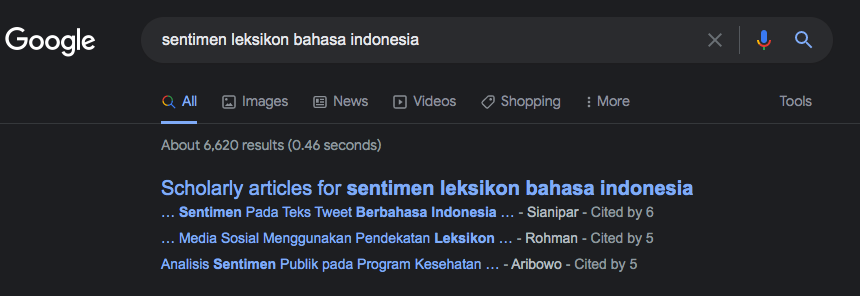
\includegraphics{images/sentimen bahasa indonesia.png}
\caption{Leksikon sentimen bahasa Indonesia}
\end{figure}

Sama dengan bahasa Inggris, leksikon untuk analisis sentimen dalam
bahasa Indonesia juga sudah banyak diteliti dengan berbagai macam
metode. Kita bisa mencari artikel ilmiah dan juga kamus nya untuk
kemudian digunakan yang salah satunya bisa didapat
\href{https://github.com/fajri91/InSet}{disini}.
\end{frame}

\hypertarget{langkah-langkah-analisis-sentimen}{%
\section{Langkah-langkah analisis
sentimen}\label{langkah-langkah-analisis-sentimen}}

\begin{frame}{Langkah-langkah analisis sentimen}
\begin{figure}
\centering
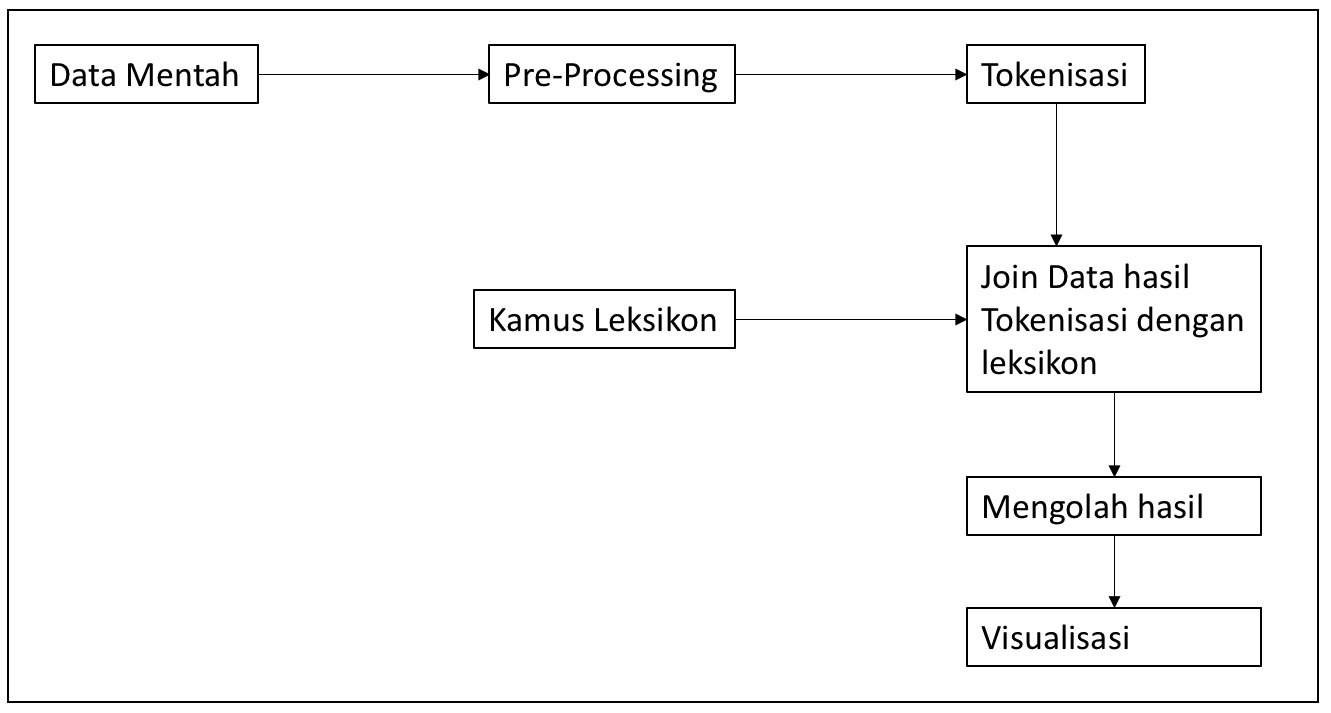
\includegraphics{images/proses sentimen.png}
\caption{Proses analisis sentimen menggunakan leksikon}
\end{figure}
\end{frame}

\hypertarget{penghitungan-sentimen}{%
\subsection{Penghitungan sentimen}\label{penghitungan-sentimen}}

\begin{frame}{Penghitungan sentimen}
\begin{figure}
\centering
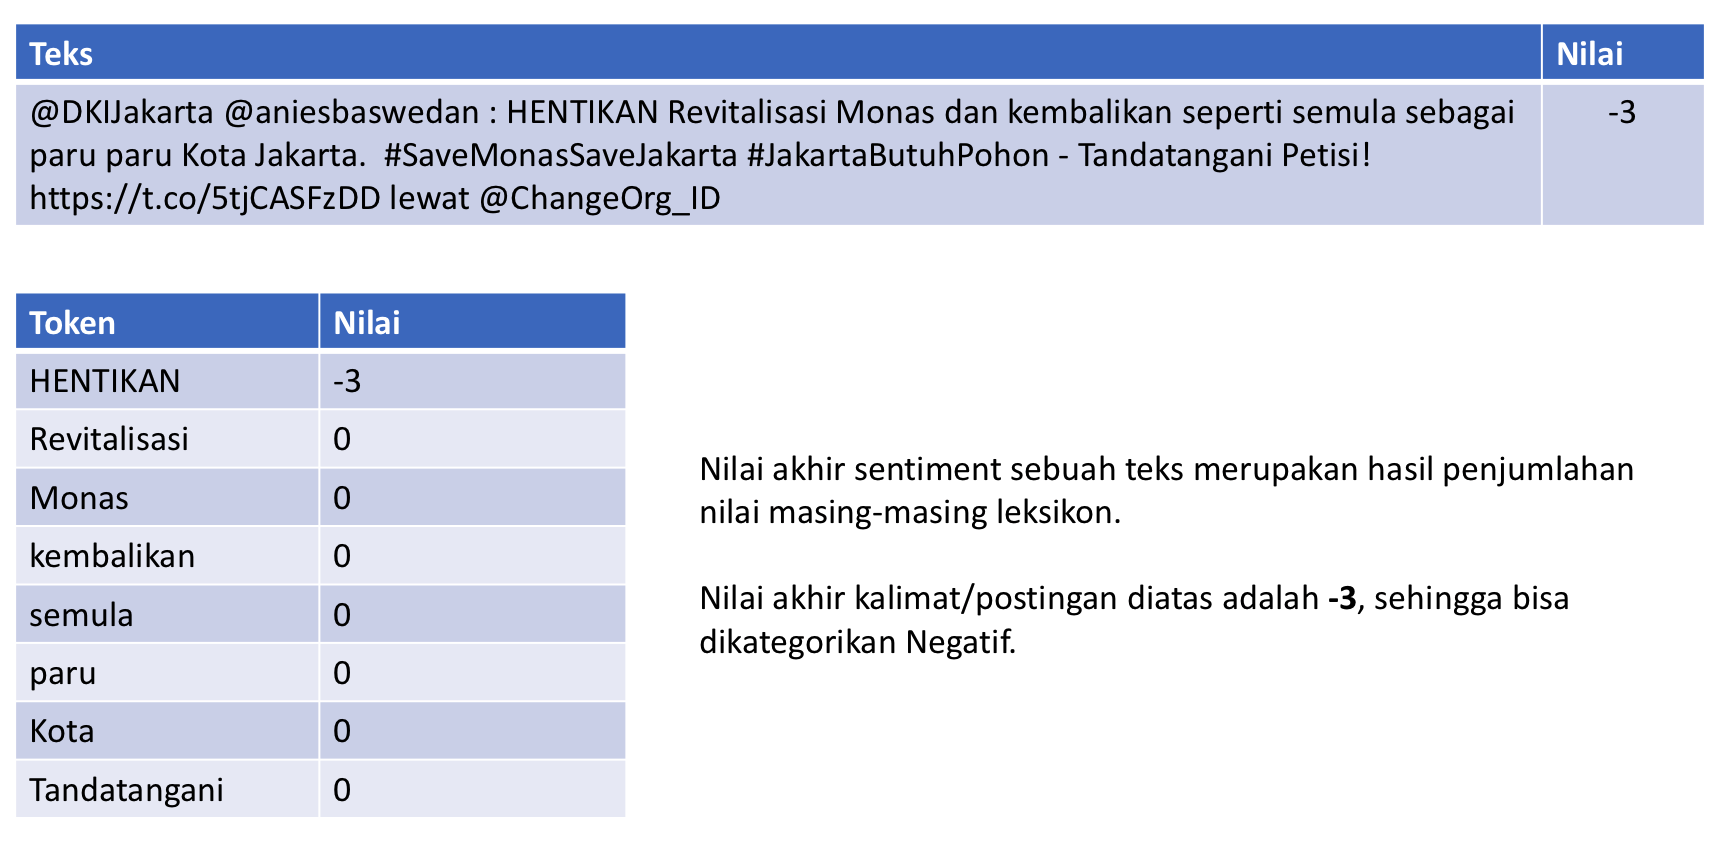
\includegraphics{images/nilai sentiment.png}
\caption{Proses sentimen menggunakan leksikon}
\end{figure}
\end{frame}

\hypertarget{persiapan}{%
\subsection{Persiapan}\label{persiapan}}

\begin{frame}[fragile]{Data yang akan dianalisis}
\protect\hypertarget{data-yang-akan-dianalisis}{}
\begin{Shaded}
\begin{Highlighting}[]
\FunctionTok{library}\NormalTok{(tidyverse)}
\FunctionTok{library}\NormalTok{(tidytext)}

\NormalTok{raw\_data }\OtherTok{=} \FunctionTok{read\_csv}\NormalTok{(}\StringTok{"data/tweet\_save\_monas.csv"}\NormalTok{)}
\NormalTok{raw\_data }\OtherTok{=}\NormalTok{ raw\_data }\SpecialCharTok{\%\textgreater{}\%} 
   \FunctionTok{select}\NormalTok{(id, created\_at, full\_text, full\_text\_clean, }
\NormalTok{          reply\_count, retweet\_count, like\_count) }\SpecialCharTok{\%\textgreater{}\%} 
   \FunctionTok{filter}\NormalTok{(}\SpecialCharTok{!}\FunctionTok{is.na}\NormalTok{(full\_text\_clean)) }\SpecialCharTok{\%\textgreater{}\%} 
   \FunctionTok{filter}\NormalTok{(}\SpecialCharTok{!}\FunctionTok{duplicated}\NormalTok{(id))}
\FunctionTok{glimpse}\NormalTok{(raw\_data)}
\end{Highlighting}
\end{Shaded}
\end{frame}

\begin{frame}[fragile]{Leksikon yang akan digunakan}
\protect\hypertarget{leksikon-yang-akan-digunakan}{}
Leksikon yang akan digunakan dapat diambil dari tautan berikut:

\begin{enumerate}
\tightlist
\item
  Leksikon Positif:
  \url{https://raw.githubusercontent.com/fajri91/InSet/master/positive.tsv}
\item
  Leksikon Negatif:
  \url{https://raw.githubusercontent.com/fajri91/InSet/master/negative.tsv}
\end{enumerate}

\begin{Shaded}
\begin{Highlighting}[]
\FunctionTok{library}\NormalTok{(tidyverse)}

\NormalTok{id\_pos }\OtherTok{=} \FunctionTok{read\_tsv}\NormalTok{(}\StringTok{"ganti dengan tautan"}\NormalTok{)}
\NormalTok{id\_neg }\OtherTok{=} \FunctionTok{read\_tsv}\NormalTok{(}\StringTok{"ganti dengan tautan"}\NormalTok{)}
\NormalTok{id\_sentimen }\OtherTok{=} \FunctionTok{bind\_rows}\NormalTok{(id\_pos, id\_neg)}
\FunctionTok{glimpse}\NormalTok{(id\_sentimen)}
\end{Highlighting}
\end{Shaded}
\end{frame}

\begin{frame}[fragile]{Tokenisasi Data}
\protect\hypertarget{tokenisasi-data}{}
\begin{Shaded}
\begin{Highlighting}[]
\NormalTok{data\_token }\OtherTok{=}\NormalTok{ raw\_data }\SpecialCharTok{\%\textgreater{}\%} 
   \FunctionTok{group\_by}\NormalTok{(id) }\SpecialCharTok{\%\textgreater{}\%} 
   \FunctionTok{unnest\_tokens}\NormalTok{(word, full\_text\_clean, }\AttributeTok{token =} \StringTok{"words"}\NormalTok{)}

\FunctionTok{glimpse}\NormalTok{(data\_token)}
\end{Highlighting}
\end{Shaded}
\end{frame}

\begin{frame}[fragile]{Join dengan leksikon}
\protect\hypertarget{join-dengan-leksikon}{}
Setelah melakukan tokenisasi, kita bisa menggabungkan data hasil
tokenisasi dengan kamus leksikon. Sehingga data yang didapatkan adalah
data dengan nilai berupa numerik.

\begin{Shaded}
\begin{Highlighting}[]
\NormalTok{hasil }\OtherTok{=}\NormalTok{ data\_token }\SpecialCharTok{\%\textgreater{}\%} 
   \FunctionTok{inner\_join}\NormalTok{(id\_sentimen)}

\NormalTok{hasil }\OtherTok{=}\NormalTok{ hasil }\SpecialCharTok{\%\textgreater{}\%} 
   \FunctionTok{group\_by}\NormalTok{(id) }\SpecialCharTok{\%\textgreater{}\%} 
   \FunctionTok{summarise}\NormalTok{(}\AttributeTok{nilai\_akhir =} \FunctionTok{sum}\NormalTok{(weight))}

\FunctionTok{glimpse}\NormalTok{(hasil)}
\end{Highlighting}
\end{Shaded}
\end{frame}

\begin{frame}[fragile]{Join dengan data asli}
\protect\hypertarget{join-dengan-data-asli}{}
\begin{Shaded}
\begin{Highlighting}[]
\CommentTok{\# penggabungan}
\NormalTok{hasil\_akhir }\OtherTok{=}\NormalTok{ raw\_data }\SpecialCharTok{\%\textgreater{}\%} 
   \FunctionTok{left\_join}\NormalTok{(hasil)}
\CommentTok{\# nilai NA menjadi 0}
\NormalTok{hasil\_akhir}\SpecialCharTok{$}\NormalTok{nilai\_akhir[}\FunctionTok{is.na}\NormalTok{(hasil\_akhir}\SpecialCharTok{$}\NormalTok{nilai\_akhir)] }\OtherTok{=} \DecValTok{0}
\CommentTok{\# memberi label}
\NormalTok{hasil\_akhir }\OtherTok{=}\NormalTok{ hasil\_akhir }\SpecialCharTok{\%\textgreater{}\%} 
   \FunctionTok{mutate}\NormalTok{(}\AttributeTok{sentimen =} \FunctionTok{case\_when}\NormalTok{(}
\NormalTok{      nilai\_akhir }\SpecialCharTok{==} \DecValTok{0} \SpecialCharTok{\textasciitilde{}} \StringTok{"Netral"}\NormalTok{, }
\NormalTok{      nilai\_akhir }\SpecialCharTok{\textgreater{}=} \DecValTok{1} \SpecialCharTok{\textasciitilde{}} \StringTok{"Positif"}\NormalTok{, }
      \ConstantTok{TRUE} \SpecialCharTok{\textasciitilde{}} \StringTok{"Negatif"}
\NormalTok{   ))}

\FunctionTok{glimpse}\NormalTok{(hasil\_akhir)}
\FunctionTok{View}\NormalTok{(hasil\_akhir)}
\end{Highlighting}
\end{Shaded}
\end{frame}

\hypertarget{melihat-hasil}{%
\subsection{Melihat Hasil}\label{melihat-hasil}}

\begin{frame}[fragile]{Persentase sentimen}
\protect\hypertarget{persentase-sentimen}{}
\begin{Shaded}
\begin{Highlighting}[]
\NormalTok{persen\_sentimen }\OtherTok{=}\NormalTok{ hasil\_akhir }\SpecialCharTok{\%\textgreater{}\%} 
   \FunctionTok{count}\NormalTok{(sentimen) }\SpecialCharTok{\%\textgreater{}\%} 
   \FunctionTok{mutate}\NormalTok{(}\AttributeTok{persen =} \FunctionTok{round}\NormalTok{(n}\SpecialCharTok{/}\FunctionTok{sum}\NormalTok{(n)}\SpecialCharTok{*}\DecValTok{100}\NormalTok{))}

\FunctionTok{library}\NormalTok{(echarts4r)}
\NormalTok{persen\_sentimen }\SpecialCharTok{\%\textgreater{}\%} 
   \FunctionTok{e\_chart}\NormalTok{(}\AttributeTok{x =}\NormalTok{ sentimen) }\SpecialCharTok{\%\textgreater{}\%} 
   \FunctionTok{e\_pie}\NormalTok{(persen)}
\end{Highlighting}
\end{Shaded}
\end{frame}

\hypertarget{distribusi-sentimen}{%
\subsection{Distribusi Sentimen}\label{distribusi-sentimen}}

\begin{frame}[fragile]{Distribusi Sentimen}
\begin{Shaded}
\begin{Highlighting}[]
\NormalTok{distribusi\_sentimen }\OtherTok{=}\NormalTok{ hasil\_akhir }\SpecialCharTok{\%\textgreater{}\%} 
   \FunctionTok{separate}\NormalTok{(created\_at, }\AttributeTok{into =} \FunctionTok{c}\NormalTok{(}\StringTok{"created\_at"}\NormalTok{, }\StringTok{"jam"}\NormalTok{), }\AttributeTok{sep =} \StringTok{" "}\NormalTok{) }\SpecialCharTok{\%\textgreater{}\%} 
   \FunctionTok{group\_by}\NormalTok{(created\_at) }\SpecialCharTok{\%\textgreater{}\%} 
   \FunctionTok{count}\NormalTok{(sentimen)}

\NormalTok{distribusi\_sentimen}\SpecialCharTok{$}\NormalTok{created\_at }\OtherTok{=} 
   \FunctionTok{as.Date}\NormalTok{(distribusi\_sentimen}\SpecialCharTok{$}\NormalTok{created\_at)}
\FunctionTok{glimpse}\NormalTok{(distribusi\_sentimen)}

\NormalTok{distribusi\_sentimen }\SpecialCharTok{\%\textgreater{}\%} 
   \FunctionTok{ggplot}\NormalTok{(}\FunctionTok{aes}\NormalTok{(}\AttributeTok{x =}\NormalTok{ created\_at, }\AttributeTok{y =}\NormalTok{ n, }\AttributeTok{color =}\NormalTok{ sentimen)) }\SpecialCharTok{+} 
   \FunctionTok{geom\_line}\NormalTok{()}
\end{Highlighting}
\end{Shaded}
\end{frame}


\section[]{}
\frame{\small \frametitle{Table of Contents}
\tableofcontents}
\end{document}
